\chapter{Fundamentos y selección de herramientas\label{FunAndTools}}
%RGM:NUEVO
En esta sección vamos a realizar una breve introducción al
paradigma conocido como Big Data. Tras esto, veremos qué
modelos de arquitecturas propone este paradigma. Para
terminar con este capítulo, haremos un breve análisis de
las distintas herramientas disponibles para que encajen con
esta arquitectura, proponiendo, finalmente, la que más se
adapte a nuestros objetivos.

\section{Big Data\label{WhatIsBigD}}

El motivo por el que se inició este nuevo paradigma del “Big Data” fue
la gran explosión de datos que tiene lugar con el surgimiento
de tecnologías como la Web 2.0, los smartphones e IoT. Se calcula que
se emiten más de 30 Terabytes de información cada segundo en el mundo
\cite{BD-2} y el IDC predice que desde 2010 a 2020 el volumen de datos
aumentará por 50 llegando por encima del Zettabyte de datos
\cite{BD-2}. Por tanto, este nuevo paradigma surge debido a que los
paradigmas tradicionales no tenían la capacidad de dar una respuesta
al manejo de grandes volúmenes de datos.

En 2001, Doug Laney describe el Big Data mediante los siguientes términos
conocidos como las 3 Vs del Big Data \cite{BD-4}:

\begin{itemize}
\item Volumen: El conjunto de datos debe ser grande.
\item Velocidad: Debe existir una forma rápida de que lleguen los datos,
  procesarlos y devolverlos.
\item Variedad: Los datos pueden ser de cualquier tipo ya sea alfanumérico,
  imágenes, sonidos, videos, etc…
\end{itemize}

No obstante, a día de hoy, IBM introdujo la cuarta V del Big Data que se
define como Veracidad, es decir, que los datos sean lo más reales posible,
ya que cuando manejamos esta cantidad de datos, encontrar datos erróneos se
hace más probable. Esto quiere decir que en Big Data nos encontramos el
gran reto de gestionar gran cantidad de datos de una forma óptima
\cite{BD-5}.

Por otra parte, encontramos tres formas de tratar los datos según las
diferentes necesidades que aparecen. A la hora de analizar los datos
debemos tener en cuenta si se procesarán los datos del pasado, lo que
implicaría reportes analíticos, entre otras aplicaciones; si se procesan en
tiempo real, lo que quiere decir que se debe mostrar lo que pasa en el
momento, y si queremos saber lo que pasará en el futuro, lo que implica
procesos de machine learning entre otros \cite{BD-3}.

Por otro lado, encontramos un cambio sustancial en las herramientas que
pertenecen a este paradigma. Esto ha dado lugar a las siguientes
características que han hecho tan popular el concepto de Big Data
\cite{BD-6}:

\begin{itemize}
\item Las bases de datos manejan datos no estructurados, aportando mucha
  más flexibilidad y dando lugar a las bases de datos NoSQL.
\item El hecho de almacenar los datos en una sola máquina suponía un mayor
  gasto económico y dificultad en su propia administración, lo que supuso
  que surgiera el concepto de escalabilidad horizontal de los datos. Este
  concepto implica que los datos no se almacenan en una sola máquina, sino
  que se distribuyen horizontalmente entre varias máquinas. Para añadir
  seguridad a estas bases de datos distribuidas, debe existir una
  redundancia de datos que son repartidos en cada máquina, dando lugar a
  que cada una de ellas tenga una pequeña copia de otra para poder
  recuperarse.
\item Siguiendo con el punto anterior, se debe escalar horizontalmente el
  procesamiento de los datos. Esto implica una coordinación absoluta entre
  las diferentes máquinas que alojan los datos y los procesan para
  devolverlos procesados a un nodo líder del cluster y que sea capaz de
  devolver, rápidamente, los datos procesados.
\item Finalmente, tras obtener los datos, los usuarios desean que se pueda
  visualizar fácilmente la información recogida. Para que dicha cantidad de
  datos sea más fácil de entender, se pueden mostrar en diferentes
  gráficas aplicando diversas ecuaciones estadísticas significativas si
  fuera necesario. El hecho de que este paradigma maneja gran cantidad de
  datos ha favorecido el desarrollo de herramientas de visualización de
  datos.
\end{itemize}


\section{Selección del modelo de arquitectura\label{arqSelect}}
%RGM:MODIFICADO DE AQUI PARA ABAJO
A la hora de seleccionar la arquitectura, seleccionaremos la que mejor se
adapte a la casuística de nuestro problema. Por un lado, tenemos la
arquitectura Kappa, la cual se reduce a una sola capa donde se procesan los
datos y se almacenan para posteriormente mostrarlos en la aplicación. Esto
lo podemos ver en la figura \ref{arqKappa} \cite{LambdaKappa2}. Por otro
lado, la arquitectura Lambda lanza dos líneas, una para los datos que se
han de mostrar rápidamente y otra para los datos de los cuales necesitamos
un procesamiento más sofisticado. Esto podemos verlo en la figura
\ref{arqLambda} \cite{LambdaKappa}. Vista la casuística del problema se
propone, una arquitectura Lambda frente a una arquitectura Kappa.
La arquitectura Lambda, nos permitirá realizar diferentes
procesamientos en tiempo real por un lado, mientras que por otro,
podremos dejar programados trabajos más costosos, como análisis
históricos,  sin penalizar el rendimiento.

Por último en este apartado, decir que dada la arquitectura
seleccionada necesitaremos seleccionar varios tipos de
herramientas. Para repartir la carga de los mensajes enviados/recibidos
necesitaremos un distribuidor de los diferentes datos que recibamos ({\em
  broker}). Tras recibir el dato necesitamos que el {\em speed layer}
realice el procesamiento en tiempo real necesitaremos con una tecnología de
Streaming que nos permita obtener del dato en bruto, la parte que nos
interesa. Por otro lado, el {\em batch layer} nos debe permitir almacenar y
consultar cualquier dato en cualquier momento ya sea en una o varias bases
de datos. Para procesar los datos posteriormente necesitamos un sistema de
{\em batching} que vaya haciendo resúmenes y obteniendo estadísticas, esto
se almacenará en el {\em serving layer}. Finalmente, para poder mostrar
dichos datos, necesitamos una plataforma de dashboard que nos ayude a
mostrar los datos en tiempo real y los post-procesados, a la cual podamos
añadir futuros informes.

\begin{figure}[htp]
\centering
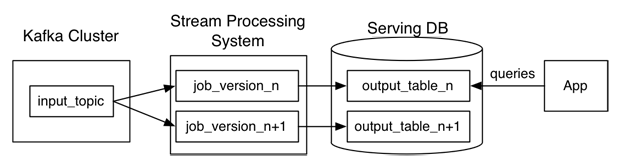
\includegraphics[scale=0.70]{Imagenes/arq1.png}
\caption{Arquitectura Kappa.}
\label{arqKappa}
\end{figure}

\begin{figure}[htp]
\centering
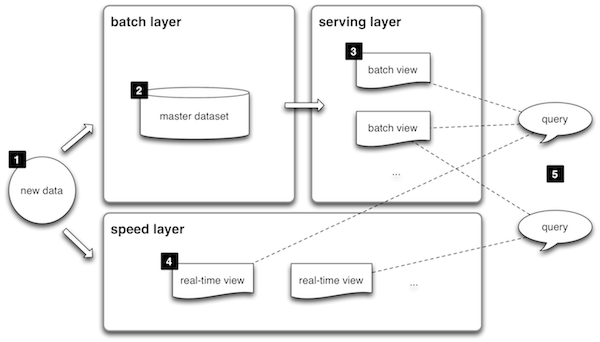
\includegraphics[scale=0.70]{Imagenes/arq2.png}
\caption{Arquitectura Lambda.}
\label{arqLambda}
\end{figure}

\section{Selección de herramientas\label{toolSelect}}

\subsection{Herramientas de virtualización\label{hvirt}}
Debido a la casuística del hardware en el que realizaremos el desarrollo y
para conseguir un sistema totalmente portable se ha decidido usar Docker
como herramienta de virtualización de los diferentes servicios. De
esta forma usaremos menos recursos a la hora de lanzar los diferentes
servicios y siendo, aún así, totalmente independientes. Por otra parte, 
Docker nos va a permitir encapsular los diferentes servicios para que puedan
ejecutarse desde cualquier máquina. Aun habiendo elegido este sistema 
también se ha valorado el uso de un Datacenter Manager como Mesos o Ambari
\cite{Hrr-1}, pero resulta ser muy pesado para el hardware que disponemos.

Por último, vamos a comentar por qué hemos elegido Docker frente a otras
posibilidades, como son las maquinas virtuales. Aunque algunas empresas
nos recomiendan subcontratar los nuevos proyectos relacionados con
tecnologías de Big Data en vez de hacer un proyecto DIY (Do It Yourself) 
\cite{Dck-14}, dada la naturaleza de nuestro trabajo, Docker es la mejor
opción. Docker nos ofrece ventajas tales como replicar y modificar las
máquinas fácilmente, podemos usarlo desde cualquier máquina descargando
la imagen directamente de Docker Hub y, posteriormente, poder probarlo en
la nube sin tener que realizar grandes modificaciones.De esta forma,
realizar cualquier cambio no requiere hacer copias de una máquina virtual
completa, sino que unicamente tendremos que modificar el fichero de 
configuración de la máquina correspondiente. En la figura 
\ref{dock-2} \cite{Dck-15} podemos comprobar que el rendimiento que se
obtiene con Docker es mejor que el de usar una máquina virtual KVM tanto
para el arranque de las máquinas como para el benchmark UnixBench
\cite{Dck-15}. En concreto, obtenemos un 30\% más de rendimiento con
Docker que con KVM aunque, evidentemente, lo mejor es ejecutarlo sobre
el hardware directamente (\emph{baremetal}). También podemos comprobar en
la figura \ref{dock-3} \cite{Dck-15} que el tiempo que tarda en arrancar
una máquina Docker es de 5 segundos, mientras que una máquina virtual KVM
tarda 15 segundos.

\begin{figure}[htp]
\centering
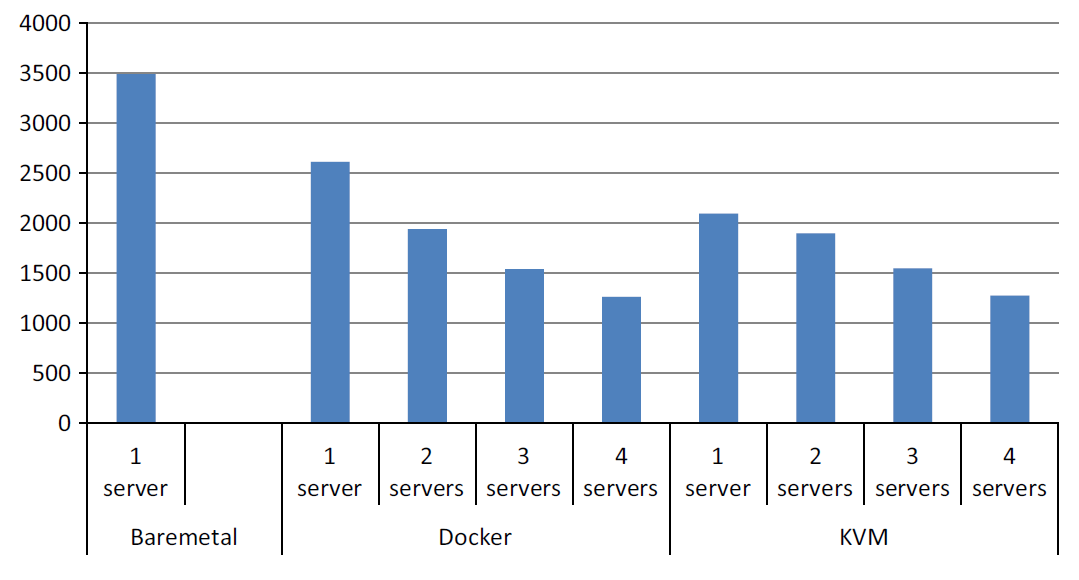
\includegraphics[scale=0.30]{Imagenes/dockervsvm2.png}
\caption{Rendimiento del benchmark con el índice UnixBench para el software
  sobre una máquina real, sobre Docker y sobre KVM.}
\label{dock-2}
\end{figure}

\begin{figure}[htp]
\centering
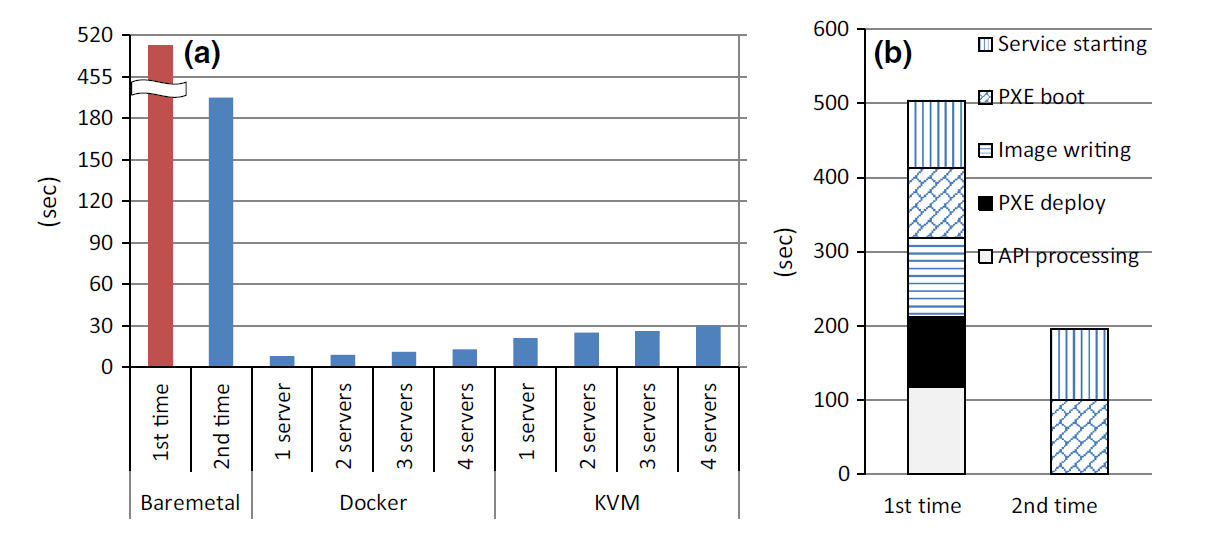
\includegraphics[scale=0.40]{Imagenes/dockervsvm3.png}
\caption{Tiempo de arranque sobre una máquina real, sobre Docker y sobre
  KVM.}
\label{dock-3}
\end{figure}

\subsection{Herramientas para el broker de mensajes\label{hbrok}}

En cuanto al \emph{broker} de mensajes, tenemos dos candidatos que son 
Apache Kafka y RabbitMQ. RabbitMQ consiste en un sistema de colas
tradicional donde encontramos un productor del mensaje y un consumidor del
mensaje y diferentes colas a las que se pueden suscribir diferentes
productores y consumidores. Por el contrario, en Apache Kafka, encontramos
que hay un productor del mensaje y varios consumidores del mismo, lo que implica
que el mensaje persistente un cierto tiempo. Podemos ver el funcionamiento
de ambos en la figura \ref{brokers-img}. Dado que, además de usarlo
como \emph{broker} también podemos usar Apache Kafka como caché, nos puede ser
útil para recuperar datos y poder operar fácilmente con las diferentes capas
que se proponen en una arquitectura Lambada. Dado esto, seleccionaremos 
como broker a Apache Kafka \cite{Hrr-2}.

\begin{figure}[htp]
\centering
\subfigure{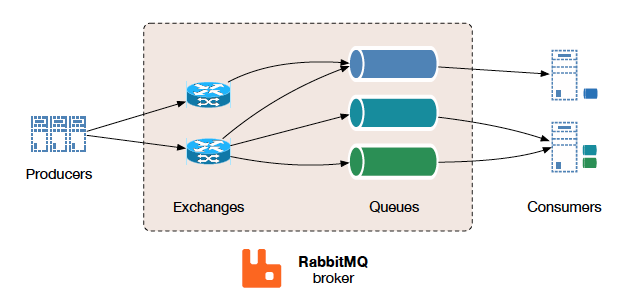
\includegraphics[width=80mm]{Imagenes/broker1.png}}
\subfigure{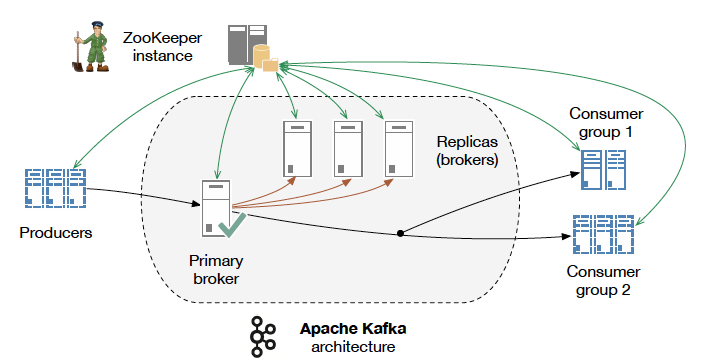
\includegraphics[width=80mm]{Imagenes/broker2.png}}
\caption{Funcionamiento de RabbitMQ y Apache Kafka}
\label{brokers-img}
\end{figure}

\subsection{Herramientas para el almacenamiento y batching\label{hbach}}

En cuanto a la parte de almacenamiento a gran escala de los datos nos
decantamos por Apache Hadoop, dada la potencia que tiene y la gran cantidad
de usuarios que la usan. Por otro lado, podemos seleccionar varios sistemas
para realizar el batching, como son Logstash, que pertenece al Stack de
Elastic, Apache Spark o Apache Hadoop.

En cuanto a las bases de datos tenemos la opción de usar Postgresql, pero
dado que queremos más flexibilidad nos decantamos por ver cómo usar bases
de datos NoSQL. Aun así, Postgresql tiene una potencia más que suficiente y
se puede escalar fácilmente. Por otro lado tenemos MongoDB, la base de
datos NoSQL más usada a dia de hoy, lo que la hace una muy buena opción
para seleccionarla \cite{Hrr-5}. Después de esta, podemos usar
Elasticsearch para almacenar datos, aunque sea un motor de búsquedas. Otras
alternativas serían InfluxDB que está optimizada para series temporales y
Redis, que nos resultará muy útil en cuanto a velocidad de consulta ya que
es una base de datos clave valor que almacena sus datos en memoria y
persiste a disco cada cierto tiempo. Evidentemente, la empresa tiene ya sus
bases de datos que habrá que integrar con esta estructura por lo que la
elección tiene que ser especialmente enfocada para el tiempo real. Aunque
Redis podría parecer a voz de pronto la mejor herramienta para estos casos
\cite{Hrr-6}, consume mucha memoria de la que actualmente, para realizar
esta prueba de concepto, no disponemos. Dado esto, nos enfocaremos en usar
Elasticsearch para este caso con su stack de tecnologías de forma que nos
permitan mostrar un dashboard de una forma mas rapida.

\subsection{Herramientas para el procesamiento en streaming\label{hspeed}}

En cuanto al {\em speed layer} encontramos diferentes tecnologías como
son Apache Spark, Apache Flink o Apache Apex. Apache Spark es un sistema
de microbaching, Apache Flink es un sistema de streaming puro y Apache Apex
es una nueva tecnología de streaming que está surgiendo en la Apache
Foundation. Dado que Apex es una tecnología que aún no está madura la
descartamos y nos tendremos que decidir entre Apache Spark y Apache Flink.
En cuanto a la integración con otras herramientas he de destacar que ambas
herramientas presentan gran compatibilidad para interoperar con Apache Hadoop.
Por otro lado, sabemos que Apache Spark trabaja en órdenes de segundos, 
ya que es {\em microbaching}, mientras que Apache Flink trabaja en el orden 
de microsegundos. Aunque Apache Flink trabaja con tiempos más pequeños
\cite{Hrr-4}, realmente no necesitamos tanta precisión en cuanto al tiempo
en streaming lo que nos hace, finalmente, decidirnos por Apache Spark
dada la gran comunidad que existe entorno a esta tecnología. Por otro
lado, la cantidad de librerías que lo componen tienen es de una gran variedad
de funciones y sus desarrolladores tienen más experiencia esto hace que sea
la herramienta más versátil para cumplir con los objetivos \cite{Hrr-3}.

\subsection{Herramientas de visualización\label{hvisual}}

En cuanto a la parte de visualización en tiempo real tenemos varias
posibilidades como son Kibana con el Stack de Elastic, Grafana, que
se integra muy bien con InfluxDB, o una web realizada a mano con D3. Dado que
hemos seleccionado, entre otras herramientas, Elasticsearch en la sección
\ref{hbach} y dada la facilidad de usar Kibana, es la herramienta elegida.


%%% Local variables:
%%% TeX-master: "main.tex"
%%% coding: utf-8
%%% ispell-local-dictionary: "spanish"
%%% TeX-parse-self: t
%%% TeX-auto-save: t
%%% fill-column: 75
%%% End:
